\documentclass[11pt]{standalone}
\usepackage{amssymb}
\usepackage{amsmath}
\usepackage[no-math]{fontspec}
\usepackage{unicode-math}
\usepackage{libertinus}
\usepackage{pgf,xcolor}
\usepackage{tikz}
\usetikzlibrary{arrows.meta, backgrounds}
\usepackage{pgfplots}
\pgfplotsset{compat=newest}

\definecolor{my_darkgray}{HTML}{484949}
\definecolor{my_lightgray}{HTML}{F3F4F4}
\definecolor{my_darkblue}{HTML}{005A94}
\definecolor{my_lightblue}{HTML}{CCDEE9}
\definecolor{my_yellow}{HTML}{FFEC7F}
\definecolor{my_red}{HTML}{E60000}
\definecolor{my_orange}{HTML}{E87846}

\begin{document}
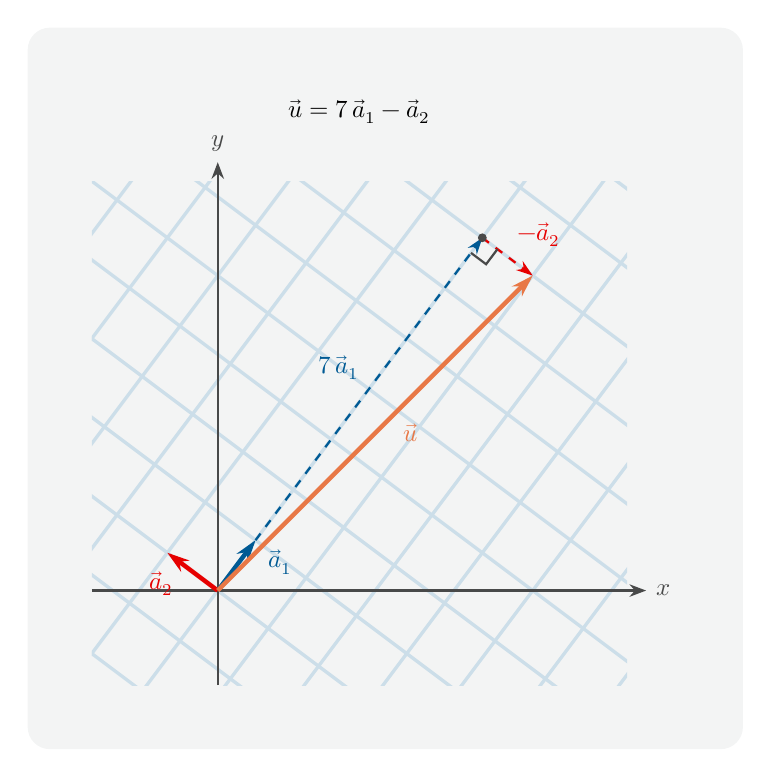
\begin{tikzpicture}[
    show background rectangle,
    background rectangle/.style={fill=my_lightgray, rounded corners=8pt},
    inner frame sep=0.8cm,
    x=0.8cm, y=0.8cm,
    vec/.style={-{Stealth[length=8pt, width=5pt]}, ultra thick},
    weg/.style={-{Stealth[length=6pt, width=4pt]}, thick, dashed}
]

% ---------------------------------------------------------------
%  Vektor u = (5, 5) in der Orthonormalbasis
%    a1 = (3, 4)/5, a2 = (-4, 3)/5,   u = 7 a1 - a2
%  Lotfusspunkt auf der Geraden durch a1: 7 a1 = (4.2, 5.6)
% ---------------------------------------------------------------

% Gitter der Orthonormalbasis: Geraden lambda_1 = k und lambda_2 = k
\begin{scope}
    \clip (-2, -1.5) rectangle (6.5, 6.5);
    \foreach \k in {-6, ..., 10} {
        \draw[my_lightblue, very thick]
            ({0.6*\k + 9.6}, {0.8*\k - 7.2}) -- ({0.6*\k - 9.6}, {0.8*\k + 7.2});
        \draw[my_lightblue, very thick]
            ({-7.2 - 0.8*\k}, {-9.6 + 0.6*\k}) -- ({7.2 - 0.8*\k}, {9.6 + 0.6*\k});
    }
\end{scope}
\draw[-{Stealth[length=6pt]}, thick, my_darkgray] (-2, 0) -- (6.8, 0)
    node[right, font=\small] {$x$};
\draw[-{Stealth[length=6pt]}, thick, my_darkgray] (0, -1.5) -- (0, 6.8)
    node[above, font=\small] {$y$};

% Weg 7 a1 - a2
\draw[weg, my_darkblue] (0.6, 0.8) -- (4.2, 5.6);
\draw[weg, my_red] (4.2, 5.6) -- (5, 5);
\node[above left, font=\small, my_darkblue] at (2.4, 3.2) {$7\,\vec{a}_1$};
\node[above right, font=\small, my_red] at (4.6, 5.3) {$-\vec{a}_2$};

% rechter Winkel im Lotfusspunkt
\draw[my_darkgray, thick] (4.02, 5.36) -- (4.26, 5.18) -- (4.44, 5.42);
\fill[my_darkgray] (4.2, 5.6) circle (1.6pt);

% Basisvektoren
\draw[vec, my_darkblue] (0, 0) -- (0.6, 0.8);
\draw[vec, my_red] (0, 0) -- (-0.8, 0.6);
\node[right, font=\small, my_darkblue] at (0.65, 0.45) {$\vec{a}_1$};
\node[below left, font=\small, my_red] at (-0.55, 0.45) {$\vec{a}_2$};

% Vektor u
\draw[vec, my_orange] (0, 0) -- (5, 5);
\node[below right, font=\small, my_orange] at (2.8, 2.8) {$\vec{u}$};

\node[font=\small] at (2.25, 7.6)
    {$\vec{u} = 7\,\vec{a}_1 - \vec{a}_2$};

\end{tikzpicture}
\end{document}
